%----------------------------------------------------------------------------------------
%	PACKAGES AND OTHER DOCUMENT CONFIGURATIONS
%----------------------------------------------------------------------------------------

\documentclass[12pt]{article}
\usepackage[danish]{babel}
\usepackage{mathtools}
\usepackage[euler]{textgreek}
\usepackage[numbered,final]{mcode}
\usepackage[utf8x]{inputenc}
\usepackage{amsmath}
\usepackage{graphicx}
\usepackage[colorinlistoftodos]{todonotes}
\usepackage[toc,page]{appendix}
%\usepackage{float}
\usepackage{floatrow} % used for adding "Source" to pictures
\usepackage{hyperref} % used for hyperlinks
\usepackage[all]{hypcap}
\usepackage{bm} % used for bold inline matj
\usepackage{lipsum} % used for lorem lipsum
\usepackage[final]{pdfpages} % used for including PDF's
\usepackage{geometry}
\usepackage{listingsutf8}
\usepackage{listings}
\usepackage{color} %red, green, blue, yellow, cyan, magenta, black, white
\definecolor{mygreen}{RGB}{28,172,0} % color values Red, Green, Blue
\definecolor{mylilas}{RGB}{170,55,241}
\hypersetup{colorlinks=true, linkcolor=black}

% Page margins
\geometry{verbose,tmargin=1in,bmargin=1in,lmargin=1in,rmargin=1in,headsep=0.35in}

\begin{document}
	
	\begin{titlepage}
		
		
		
		\newcommand{\HRule}{\rule{\linewidth}{0.5mm}} % Defines a new command for the horizontal lines, change thickness here
		\setlength{\topmargin}{0in}
		\centering % Center everything on the page
		
		%----------------------------------------------------------------------------------------
		%	HEADING SECTIONS
		%----------------------------------------------------------------------------------------
		\textsc{\LARGE Aarhus universitet}\\[1.5cm] % Name of your university/college
		\textsc{\Large Indlejret Signalbehandling}\\[0.5cm] % Major heading such as course name
		\textsc{\large 6. Semester}\\[0.5cm] % Minor heading such as course title
		
		%----------------------------------------------------------------------------------------
		%	TITLE SECTION
		%----------------------------------------------------------------------------------------
		
		\HRule \\[0.4cm]
		{ \huge \bfseries ISB projekt}\\ % Title of your document
		\HRule \\[1cm]
		
		%----------------------------------------------------------------------------------------
		%	AUTHOR SECTION
		%----------------------------------------------------------------------------------------
		
		\begin{minipage}{0.4\textwidth}
			\begin{flushleft} \large
				\emph{Gruppemedlemmer:}\\
				Søren Landgrebe \\
				Stinus Lykke Skovgaard \\
			\end{flushleft}
		\end{minipage}
		~
		\begin{minipage}{0.4\textwidth}
			\begin{flushright} \large
				\emph{Studienr:} \\
				201508295\\
				201401682\
			\end{flushright}
		\end{minipage}\\[5cm]
		
		%----------------------------------------------------------------------------------------
		%	LOGO SECTION
		%----------------------------------------------------------------------------------------
		
		
\includegraphics[scale=0.5]{Img/logo.jpg}\\[1cm]
		
		%----------------------------------------------------------------------------------------
		%	DATE SECTION
		%----------------------------------------------------------------------------------------
		
		{\large \today}\\[0.5cm] % Date, change the \today to a set date if you want to be precise
		
		
		\vfill % Fill the rest of the page with whitespace
		
	\end{titlepage}
	
\newpage
\tableofcontents
\newpage
\listoffigures
\newpage

\hypersetup{linkcolor=blue}



%!TEX root = ../../Main.tex
\graphicspath{{Chapters/Indledning/}}
%-------------------------------------------------------------------------------

\chapter{Indledning}
\section{Indledning}
Under optagelse til et live madprogram, sker det ofte at værten skal bruge en blender/foodprocesser. Dette betyder at værten ikke kan kommunikere med seerne mens blenderen/foodprocesseren kører. Denne problematik vil Noise Suppression System (NSS) kunne afhjælpe. Gennem en digital signal prossesering (DSP), vil vi dæmpe støjsignalet fra en køkkenmaskine dynamisk i realtid. Systemet består af to mikrofoner, et placeres tæt på støjen, et andet tæt på værten. De to mikrofoner fungere som input til vores system (Blackfin), hvor procceseringen og filtreringen foregår. Efter proceseringen bliver produktet afspillet på en højtaler, som erstatning for højtaleren fra et tv-apperat. Et overblik over systemet kan ses på figur \ref{fig:konceptbillede}

\begin{figure}[H]
	\centering
	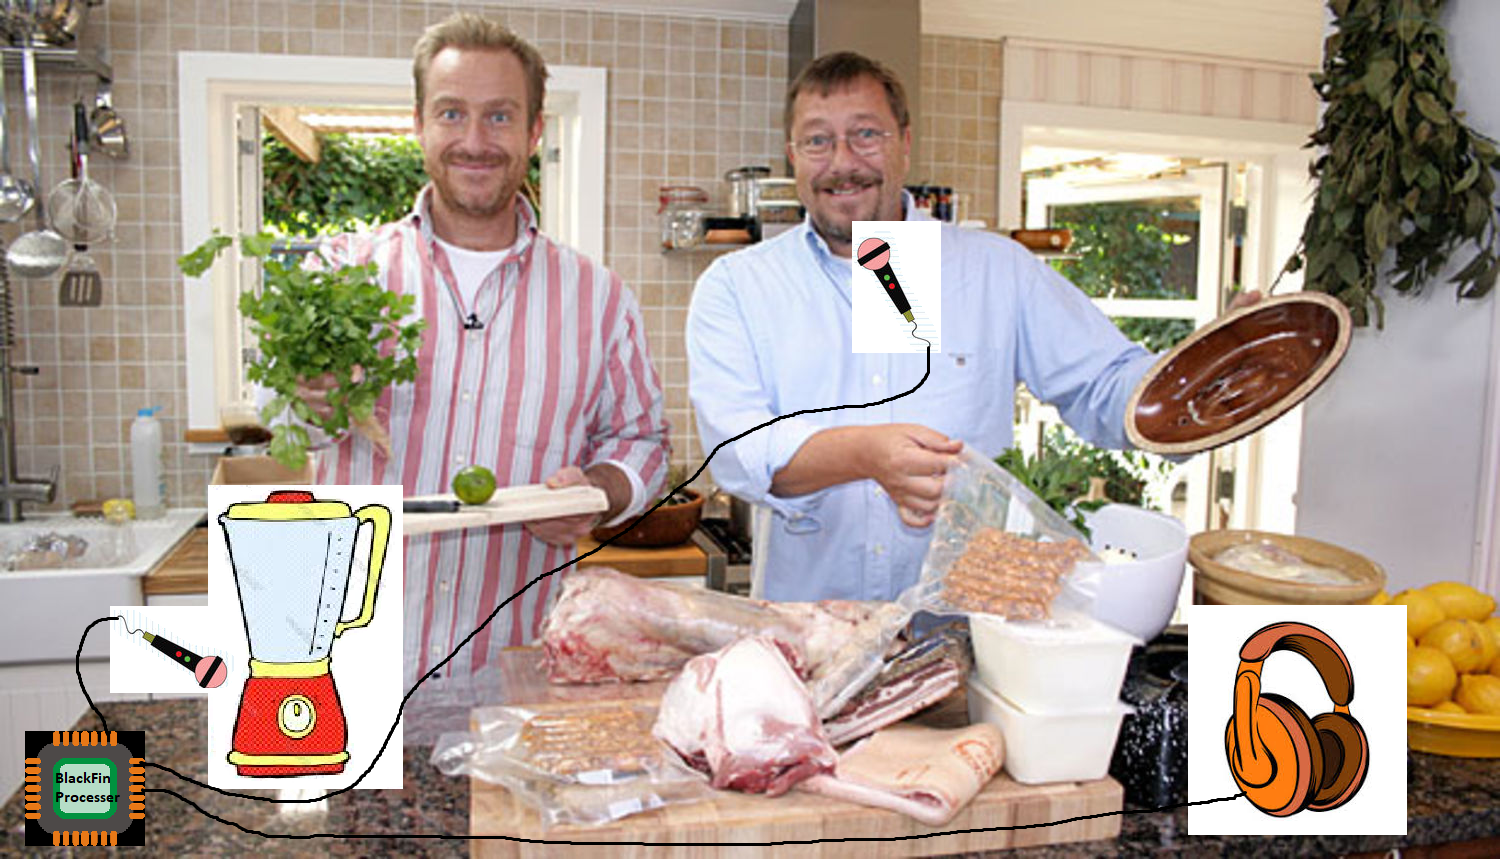
\includegraphics[width = 400pt]{Img/Konceptbillede}
	\caption{Konceptbillede for NSS}
	\label{fig:konceptbillede}
\end{figure}

Med udgangspunkt i brugerens behov vil der blive opstillet en række brugsscenarier, der beskriver brugerens interaktion med systemet. Disse scenarier vil sammen med en række veldefinerede krav og afgrænsninger, danne grundlaget for designet af alle dele af systemet.  \\ 

\newpage


	%!TEX root = ../../Main.tex
\graphicspath{{Chapters/Krav/}}
%-------------------------------------------------------------------------------


\section{Krav}
I dette afsnit beskrives kravene til hvilken funktionalitet systemet har. 


I samarbejde med vejleder er der opstillet en række krav.
\begin{itemize}
\item Systemets skal kunne filtrere en støj fra et lydsignal, som indeholder et tale signal overlappet af et støjsignal.
\item Brugeren skal manuelt kunne tænde og slukke for filtreringen.
\item Output lydsignalet skal feedes til en højtaler som afspiller lyden fra mikrofonen. 
\end{itemize}

Kravene er bygget op gennem use cases, som beskriver systemets funktionelle krav, samt en liste over alle ikke-funktionelle krav for systemet. Først vises aktørbeskrivelserne
med tilhørende aktørkontekst diagram. Herefter vises use cases for systemet. Der er udfærdiget to use cases
der tilsammen beskriver funktionaliteten af systemet. I use case afsnittet vises der også et use case diagram
med alle use cases og hvordan aktørerne interagerer med dem. Til sidst gives et kort overblik over ikke funktionelle krav.

\section{Aktørbeskrivelse}

\begin{figure}[H]
	\centering
	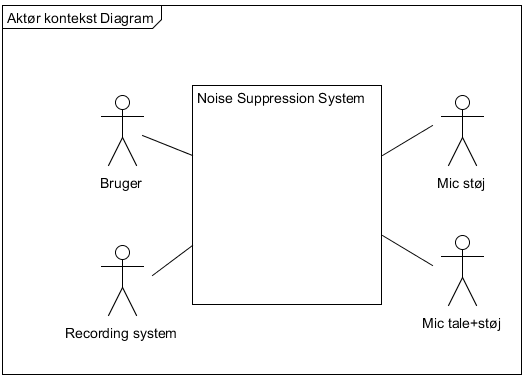
\includegraphics[width = 200 pt]{Img/Aktoer_Kontekst.png}
	\caption{Aktør Kontekst diagram}
	\label{fig:Aktoer Kontekst diagram}
\end{figure}

På figur \ref{fig:Aktoer Kontekst diagram} ses aktør kontekst diagrammet som beskriver sammenhængen mellem aktørene og det system de interagere med. Aktørene er som følger: \\*
\textbf{Primær}\\
\textbf{Bruger:} Den aktør der interagerer med systemet og vælger den ønskede funktionalitet \\
\textbf{Recording system:} Den aktør der modtager det enedelige produkt\\
\textbf{Sekundær}\\
\textbf{Mic støj:} Et input til det samlede system\\
\textbf{Mic tale+støj:} Et input til det samlede system \\

\section{Use case beskrivelse}

\begin{figure}[H]
	\centering
	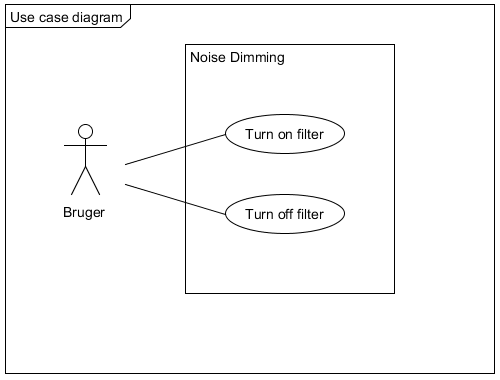
\includegraphics[width = 300 pt]{Img/Usecase_Diagram.png}
	\caption{Usecase diagram}
	\label{fig:Usecase diagram}
\end{figure}

På figur \ref{fig:Usecase diagram} ses usecase diagrammet som beskriver sammenhængen mellem aktørerne og de forskellige funktionaliteter der findes for systemet.

\subsubsection{UC 1 - Turn on filter}

Brugeren trykker på SW1 og filteret aktiveres. 


\subsubsection{UC 2 - Turn off filter}

Brugeren trykker på SW1 og filteret deaktiveres. 

\subsubsection{UC 3 - Filter aktiv}

Recording system modtager det filtrede lyd, hvis prækonditionen UC 1  er udført. 

\newpage
\section{Ikke-funktionelle krav}
Kravene er delt op i tre underkategorier. Krav der relaterer til problemet. krav der relaterer til DSP platform og algoritme. Til sidst er der en kategori der beskriver kravene til systemet på baggrund af de to første kategorier.
\begin{enumerate}
	
	\subsection{Problemrelateret krav}
	\item R1: Systemet skal have 2 mikrofoner og 1 højtaler
	
	\item R2: Filteret skal gøre brug af LMS algoritmen
	
	\item R3: Systemet skal kunne processerer lyd i frekvensbåndet 50-20000Hz. 
	
	\item R4: Systemet skal kunne dæmpe uønkset støj 30dB.
	
	\item R5: Systemet skal kunne dæmpe støj uden at dæmpe ønsket lydsignal.
	
	\item R6: Systemet burde have en latency under 30ms.
	
	\item R7: Systemet burde have et dynamikområde på min 80dB
	
	\subsection{System og algoritme krav}
	
	\item R8: Filter algoritmen skal implementeres med fixed point 
	
	\item R9: Filteret skal max bruge 10kByte memory
	
	\item R10: Filteret skal implementeres på Blackfin BF533
	
	\item R11: Filteret må max benytte 98\% DSP load

	\subsection{Afledte krav}
	
	\item DR1: DSP systemet skal kunne håndtere en samplingsrate på min 44100kHz(På baggrund af krav R3) 
	
	\item DR2: Filteret skal implementeres med 1.15 fixed point.(På baggrund af krav R7 og R8. Dette giver et dynamikområde på 96dB)
	
	\item DR3: Filter latency må max forsinkes 1280 samples(På baggrund af R6. (1/44100)*1280=30ms)
	
	\item Filteret må max bruge 13333 cycles af DSP processering for hver sample. (På baggrund af R10, R11 og DR1 (600MHz/44.1kHz)*90\%)
	
\end{enumerate}


\section{Acceptest}
Til hver use case er der lavet en tilhørende accepttest, der tjekker om use casen bliver gennemført korrekt. Udover de tre accepttests er der oprettet en accepttest af de ikke-funktionelle krav til systemet. Alle accepttests kan ses
i kravspecifikations dokumentation.
%!TEX root = ../../Main.tex
\graphicspath{{Chapters/Struktur/}}
%-------------------------------------------------------------------------------

\section{Struktur}

I dette projekt er der taget et valg udfra læringsmålene om at vi bruger Blackfin platformen til at udføre projektetes funktionalitet. Da en blackfin processor er bygget op af mange funktionalle blokke, vil der i det kommende afsnit laves et overblik over de hardware blokke som bliver brugt i dette projekt. 

\begin{figure}[H]
	\centering
	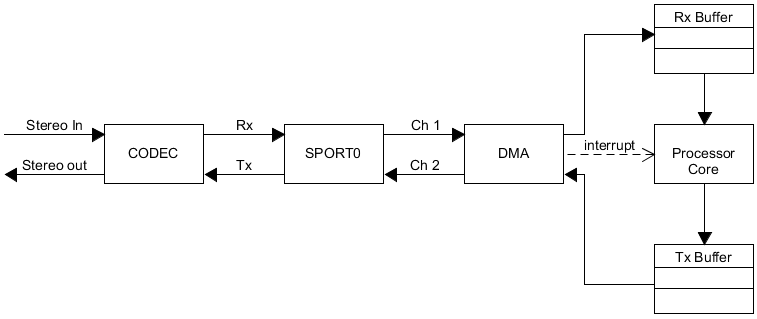
\includegraphics[width = 400pt]{Img/Struktur}
	\caption{Struktur NSS}
	\label{fig:LMS_filter}
\end{figure}

Igennem processen af vores funktionalitet, sendes lydsignalet gennem en codec1836, som har til opgave at sende inputtet gennem en ADC, hvorefter den sender det digitale signal videre til SPORT0, som står for at forbinde de interne blokke, igennem dette projekt bruger vi den interne clock, hvor frekvensen kan beregnes ud fra formlen:

\begin{figure}[H]
	\centering
	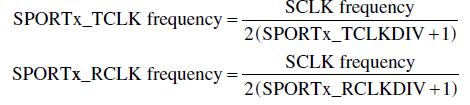
\includegraphics[width = 300pt]{Img/Frekvens}
	\caption{Formel for clock frekvens}
	\label{fig:LMS_filter}
\end{figure}
  
Systemet fører herefter signalet til DMA'en som står for at placerer dataen i de rigtige registre i memory. Herefter sker selve proceceringen af dataen, hvor vores funktionalitet er implementeret. Det filtrede og bearbejde signal sendes herefter den modsatte vej og kommer igennem alle blokke igen og ender som et analogt signal på udgangen. 

\newpage


%!TEX root = ../../Main.tex
\graphicspath{{Chapters/Teori/}}
%-------------------------------------------------------------------------------


\section{Teori}
I procceseringsfasen af projektet, har vi valgt at bruge et adaptivt filter - LMS (Least Mean square) algoritme. LMS er et adaptivt filter som består af 2 funktionelle blokke, hvor den ene blok (Linear Filter) fungerer som et filter, det andet (Adaptive Algorithm) som et dynamisk beregner af nye koefficinter til første blok.  Filteret trækker herefter de beregnede filter fra det samlede lydsignal. 
   

\begin{figure}[H]
	\centering
	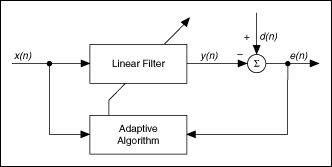
\includegraphics[width = 400pt]{Img/Figures}
	\caption{LMS adaptive filter}
	\label{fig:LMS_filter}
\end{figure}

På figur \ref{fig:LMS_filter} ses et overblik over det adative system, hvor x(n) er støjsignalet, y(n) er det filtrede støjsignal, med koefficienter som opdateres fra blokken "Adaptive Algoritm". d(n) er det ønskede signal inklusiv det støjende signal. e(n) er forskellen mellem d(n) og y(n) og derved støjen fratrukket fra det samlede signal af ønsket og støj.\cite{Teori}  \newline 


Det digitale filter bliver beregnet ud fra formlen:

\begin{equation}
  y(n) = \displaystyle\sum_{l=0}^{L-1} W(n)*x(n-1)
\end{equation}
Hvor W(n) er den værdi, som dynamisk opdateres. Dette sker ved at vi beregner den næste værdi ud fra formlen: 

\begin{equation}
  W(n+1) = W(n)-\mu *X(n)*e(n)
\end{equation}

Hvor W er den nye koefficient til filteret, X(n) er input signalet, og \textmu\ er en faktor, som bestemmer hastigheden af filteret, samt styrer infaldstiden. Hvis \textmu\ er lav bliver filteret langtsommere, mens settling time stiger jo højere vi kommer. Typisk må denne værdi ikke overstige 1. 
\newline
Dette giver os et endeligt udtryk som stemmer overens med figur \ref{fig:LMS_filter}, ift summeringspunktet: 
\begin{equation}
  e(n) = d(n)-y(n)
\end{equation} 

%!TEX root = ../../Main.tex
\graphicspath{{Chapters/Matlab/}}
%-------------------------------------------------------------------------------


\section{Matlab simulering}

Efter den teoretiske undersøgelse, vil vi i dette afsnit udvikle og vise en simuleret version af vores filter, hvor der er taget udgangspunkt i Teori afsnittet. Da vi tager udgangspunkt i teoriafsnittet starter vi med at vise hvordan vi har implementeret vores filter. 

\begin{lstlisting}
%Create LMS FIR filter
my = 0.01; % some number 0.01
W = zeros(1,256);

for n = 1:length(d) %run every sample 
    yn = 0;
    for m = 1:length(W) %make new filteret sample 
        if n > m
            yn = yn + fixed32(W(m)*noise(n-m));
        end
    end
    y(n) = yn;
    e(n) = d(n) - y(n);
    for m = 1:length(W) %make new koefficient  
        if n > m
            W(m) = W(m) + fixed32(my*noise(n-m)*e(n));
        end
    end
end
\end{lstlisting}

Først i filteret vælger vi en my, som ift til teori afsnittet bestemmer hvor hurtig filteret er. I dette eksempel bruger vi en værdi som er testet frem til at have et god forhold mellem hastighed og settling time. Herefter bestemmes hvor mange koefficienter filteret skal have. Vi har valgt et forholdsvis højt tal, da vi simulerer. Dette vil ikke nødvendigvis være muligt på Cross-core. \\

Igennem genereringen af filteret laves der 3 forloop. Et som kører hver sample igennem, et som laver det filtrede nye sample, og et som opdaterer koefficinterne ift tilbagekoblingen. \\
De nye filter koefficienter bliver herved opdateret til det ønskede filter, hvor e(n) bliver fejlen ift figur \ref{fig:LMS_filter}, som er det talesignal der ønskes. \\
Koden er bygget op sådan at vi kører en fixed16 og fixed32, for at simulere det bedst muligt ift blackfin. Fixed16 svarer til fixed point 1.15 og fixed32 til fixed point 1.31. 
\\
Dette giver os et filter som fungerer efter hensigten. Først testes der med 3 sinus toner, som ligger indover et tale signal, disse 3 toner skal derved gerne blive filtreret gennem filteret. 
\newpage
\subsection{Første test}
Den første test der blev udført var så simpel som mulig. I forsøget generes et talesignal med 3 sinustoner indover. 
Figur \ref{fig:Filter_time} viser signalet som bliver filtreret i tidsdomænet. Her er det værd at observerer settling tiden på filteret som ses i y(n). Denne settling tid vil kunne gøres mindre ved at justere på my. Der er valgt til opgaven her at teste med 0.01 my. 
\begin{figure}[H]
	\centering
	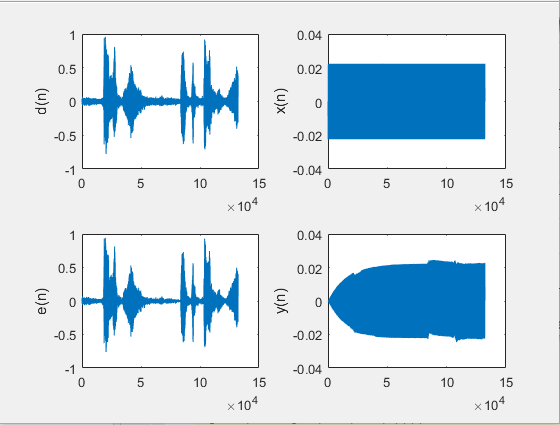
\includegraphics[width = 400pt]{Img/Filter_time}
	\caption{LMS filter i tid (3 sinus toner)}
	\label{fig:Filter_time}
\end{figure}
\newpage
Herefter vises på figur \ref{fig:Filter_Freq} signalet i frekvens domænet, her ses hvordan filteret filtrere den fejl som skabes fra, og derved skaber et signal e(n), som er talesignalet uden sinus tonerne. 

\begin{figure}[H]
	\centering
	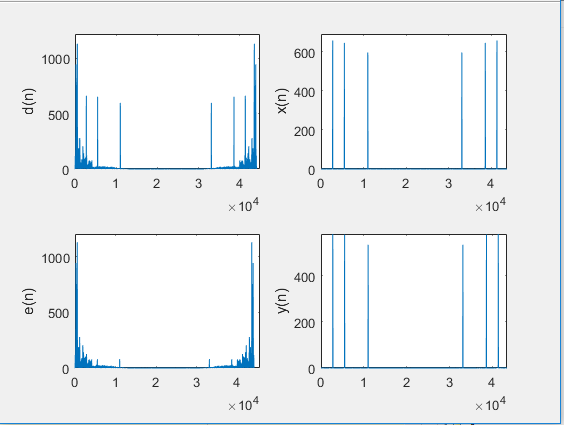
\includegraphics[width = 400pt]{Img/Filter_Freq}
	\caption{LMS filter i frekvens (3 sinus toner)}
	\label{fig:Filter_Freq}
\end{figure}
\newpage
Ved at kigge på selve filteret ses at filteret (figur \ref{fig:Filter}) skaber et filter som kune lukker de 3 sinus toner igennem, hvilket er hensigten. Dette signal bliver så fratrukket det endelige samlede signal, for at få en error som er det endelige e(n). 
\begin{figure}[H]
	\centering
	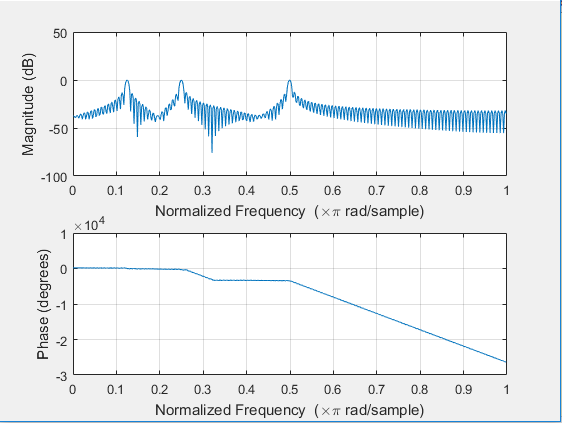
\includegraphics[width = 400pt]{Img/Filter}
	\caption{LMS filter(3 sinus toner)}
	\label{fig:Filter}
\end{figure}
\newpage
\subsection{Anden test}
Første test var i den nemme og simple ende, da vi kun skulle filtrere rene toner fra, vil der i anden test forsøges at filtere en foodprocessor som bekrevet i indledningen. Denne opgave en del mere udfordrende for filteret da den nu skal filtrere på mange toner og ikke kune 3, samtidig med den skal lade nogle bestemte toner gå igennem, som kommer fra talesignalet. \\
På figur \ref{fig:Filter_time_food}, ses nu det endelige produkt i tidsdomænet, der ses her en kraftig filtrering af signalet fra d(n) til e(n). Igen ser vi også en y(n) der har en settling time, inden filteret begynder at virke efter hensigten. 

\begin{figure}[H]
	\centering
	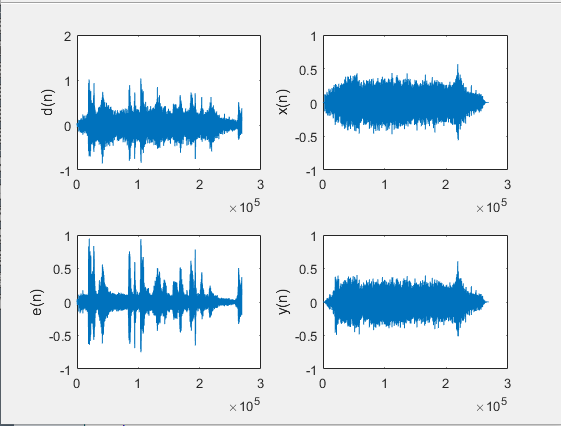
\includegraphics[width = 400pt]{Img/Filter_time_food}
	\caption{LMS filter i tid (food processor)}
	\label{fig:Filter_time_food}
\end{figure}
\newpage

Herefter tager vi et blik på frekvens donænet som viser lidt det samme billede som tidsdomænet, at LMS filteret filtrerer kraftigt fra d(n) til e(n), dette kommer af at foodprocessoren er indeholder mange lydfrekvenser. Hvis vi kigger lidt på figur \ref{fig:Filter_Freq_food}, og figur \ref{fig:Filter_food}, kan man nærstudere figur \ref{fig:Filter_food}, og se at filteret fungerer bedst når frekvenserne er udenfor talefrekvenserne, dette betyder også at filteret ikke prøve at filtrere støj fra som ligger i tale signalet, dette kan vi se fra figur \ref{fig:Filter_food}.

\begin{figure}[H]
	\centering
	\includegraphics[width = 400pt]{Img/Filter_Freq_food}
	\caption{LMS filter i frekvens (food processor)}
	\label{fig:Filter_Freq_food}
\end{figure}
\newpage

\begin{figure}[H]
	\centering
	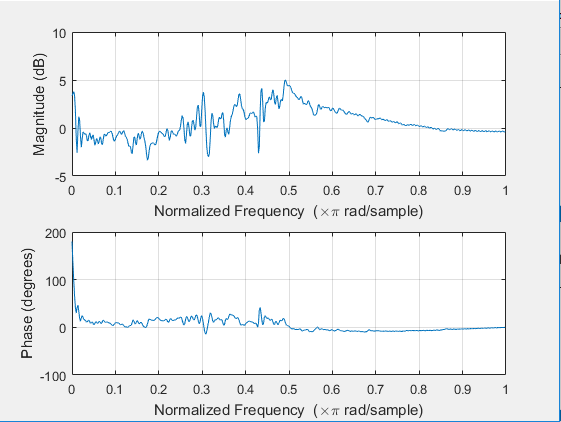
\includegraphics[width = 400pt]{Img/Filter_food}
	\caption{LMS filter(food processor)}
	\label{fig:Filter_food}
\end{figure}





\begin{flushleft}
	
\end{flushleft}


\bibliographystyle{plain}
\bibliography{Bibliography}	

\begin{thebibliography}{9}

\bibitem{Teori} 
Gan and Kuo. \\
\textit{Embedded Signal Processing with the Micro Signal Architecture, Chapter 4.4.1}\\ 
John Wiley 1st Ed. 2007.
 
\bibitem{Struktur} 
Gan and Kuo. \\
\textit{Embedded Signal Processing with the Micro Signal Architecture, Chapter 7.2.2.1}\\ 
John Wiley 1st Ed. 2007.
  
\end{thebibliography}

\end{document}